% Created 2021-07-23 Fri 15:33
% Intended LaTeX compiler: pdflatex
\documentclass[a4paper]{article}
\usepackage[utf8]{inputenc}
\usepackage[T1]{fontenc}
\usepackage{graphicx}
\usepackage{grffile}
\usepackage{longtable}
\usepackage{wrapfig}
\usepackage{rotating}
\usepackage[normalem]{ulem}
\usepackage{amsmath}
\usepackage{textcomp}
\usepackage{amssymb}
\usepackage{capt-of}
\usepackage{hyperref}
\author{Emilio Depero}
\date{\today}
\title{Old list from Dipanwita}
\hypersetup{
 pdfauthor={Emilio Depero},
 pdftitle={Micromegas instruction 2018},
 pdfkeywords={},
 pdfsubject={},
 pdfcreator={Emacs 27.2 (Org mode 9.4.5)}, 
 pdflang={English}}
\begin{document}

\maketitle
\section{MM shift instruction}
\label{sec:org331ae60}
\subsection{General monitoring}
\label{sec:org71544ff}
The MicroMegas can be monitored using the COOOL software:
\begin{enumerate}
\item type in the terminal \$StartCOOOL.sh
\item Open the config file /home/daq/MM.cfg to look at the profiles
\item After 50 spills save a ps immage using config file /home/daq/SHIFT\textsubscript{MM.cfg} in the folder /home/emilio/MMruns with name MM\_<run number>
\end{enumerate}
\textbf{NOTE}  : The geometry of MM1,MM3,MM4 and MM6 is rotated by 90 degree within respect to the one of the other MicroMegas, that show the beam spot as an observer standing in front of them would see it,
this is the reason they look rotated in COOOL

\subsection{Voltage and current monitoring}
\label{sec:org9ca0442}
All MicroMegas should have 0-5 nA current (can be occasionaly a bit larger for some modules, not above 10 nA) on both power supply channel off spill
and some current during the spill on channel B (resistive strips). It is important to check that the current correctly
goes back to zero between two spills in Slow Control. If not the accumulated current might bring the
detector to breakdown.
\subsection{Gas monitoring}
\label{sec:orga03a7b6}
The value of the pressure of the gas bottle connected to the \uline{red gas pipe} and attached label with the name \uline{Emilio Depero} on it. 
should be monitored (ideally by making a photo and put it on the ELOG) at the beginning and at the end of every shift. If the values
of the first manometer (the one closer to the gas bottle) drop lower than 30 Bar contact one of the MM responsable.
\subsection{Troubleshooting}
\label{sec:org8db427d}
\subsubsection{MM are not loading}
\label{sec:org94c1fd3}
It happens quite a lot that MM need to be loaded more then once. Type:

\begin{itemize}
\item LOAD -A 622
\end{itemize}

at least 3-4 times before giving up. If it doesn't work try to type the following
command in order:

\begin{itemize}
\item LOAD -g 622
\item LOAD -zR 622
\item LOAD -ra 622
\item LOAD -p 622

This can sometime works when the command LOAD -A 622 does not work. If you get error immediately and consistently after typing
LOAD -zR 622 or LOAD -g 622 there are two possible solutions:
\item switch off the ADCGemFull in the database (\url{http://pcdmfs01.cern.ch/}). Type LOAD -A 622 one more time, if it works, switch on ADCGemFull one more time and try to load again. This has proven to work in the past.
\item ADC need a power cycle. This can done automatically using the slow control software on the windows desktop on the left corner of the controlroom with name DCS PCCOMPASS010:
\textbf{username} = PCCOMPASS010
\textbf{password} = Na642018
Then click on the GEM button, the LV System and finally on the OFF button of both of the power supply windows. Wait for one minute all channel to show OFF, then click ON on both of the windows to turn
them on again.
\end{itemize}
\begin{center}
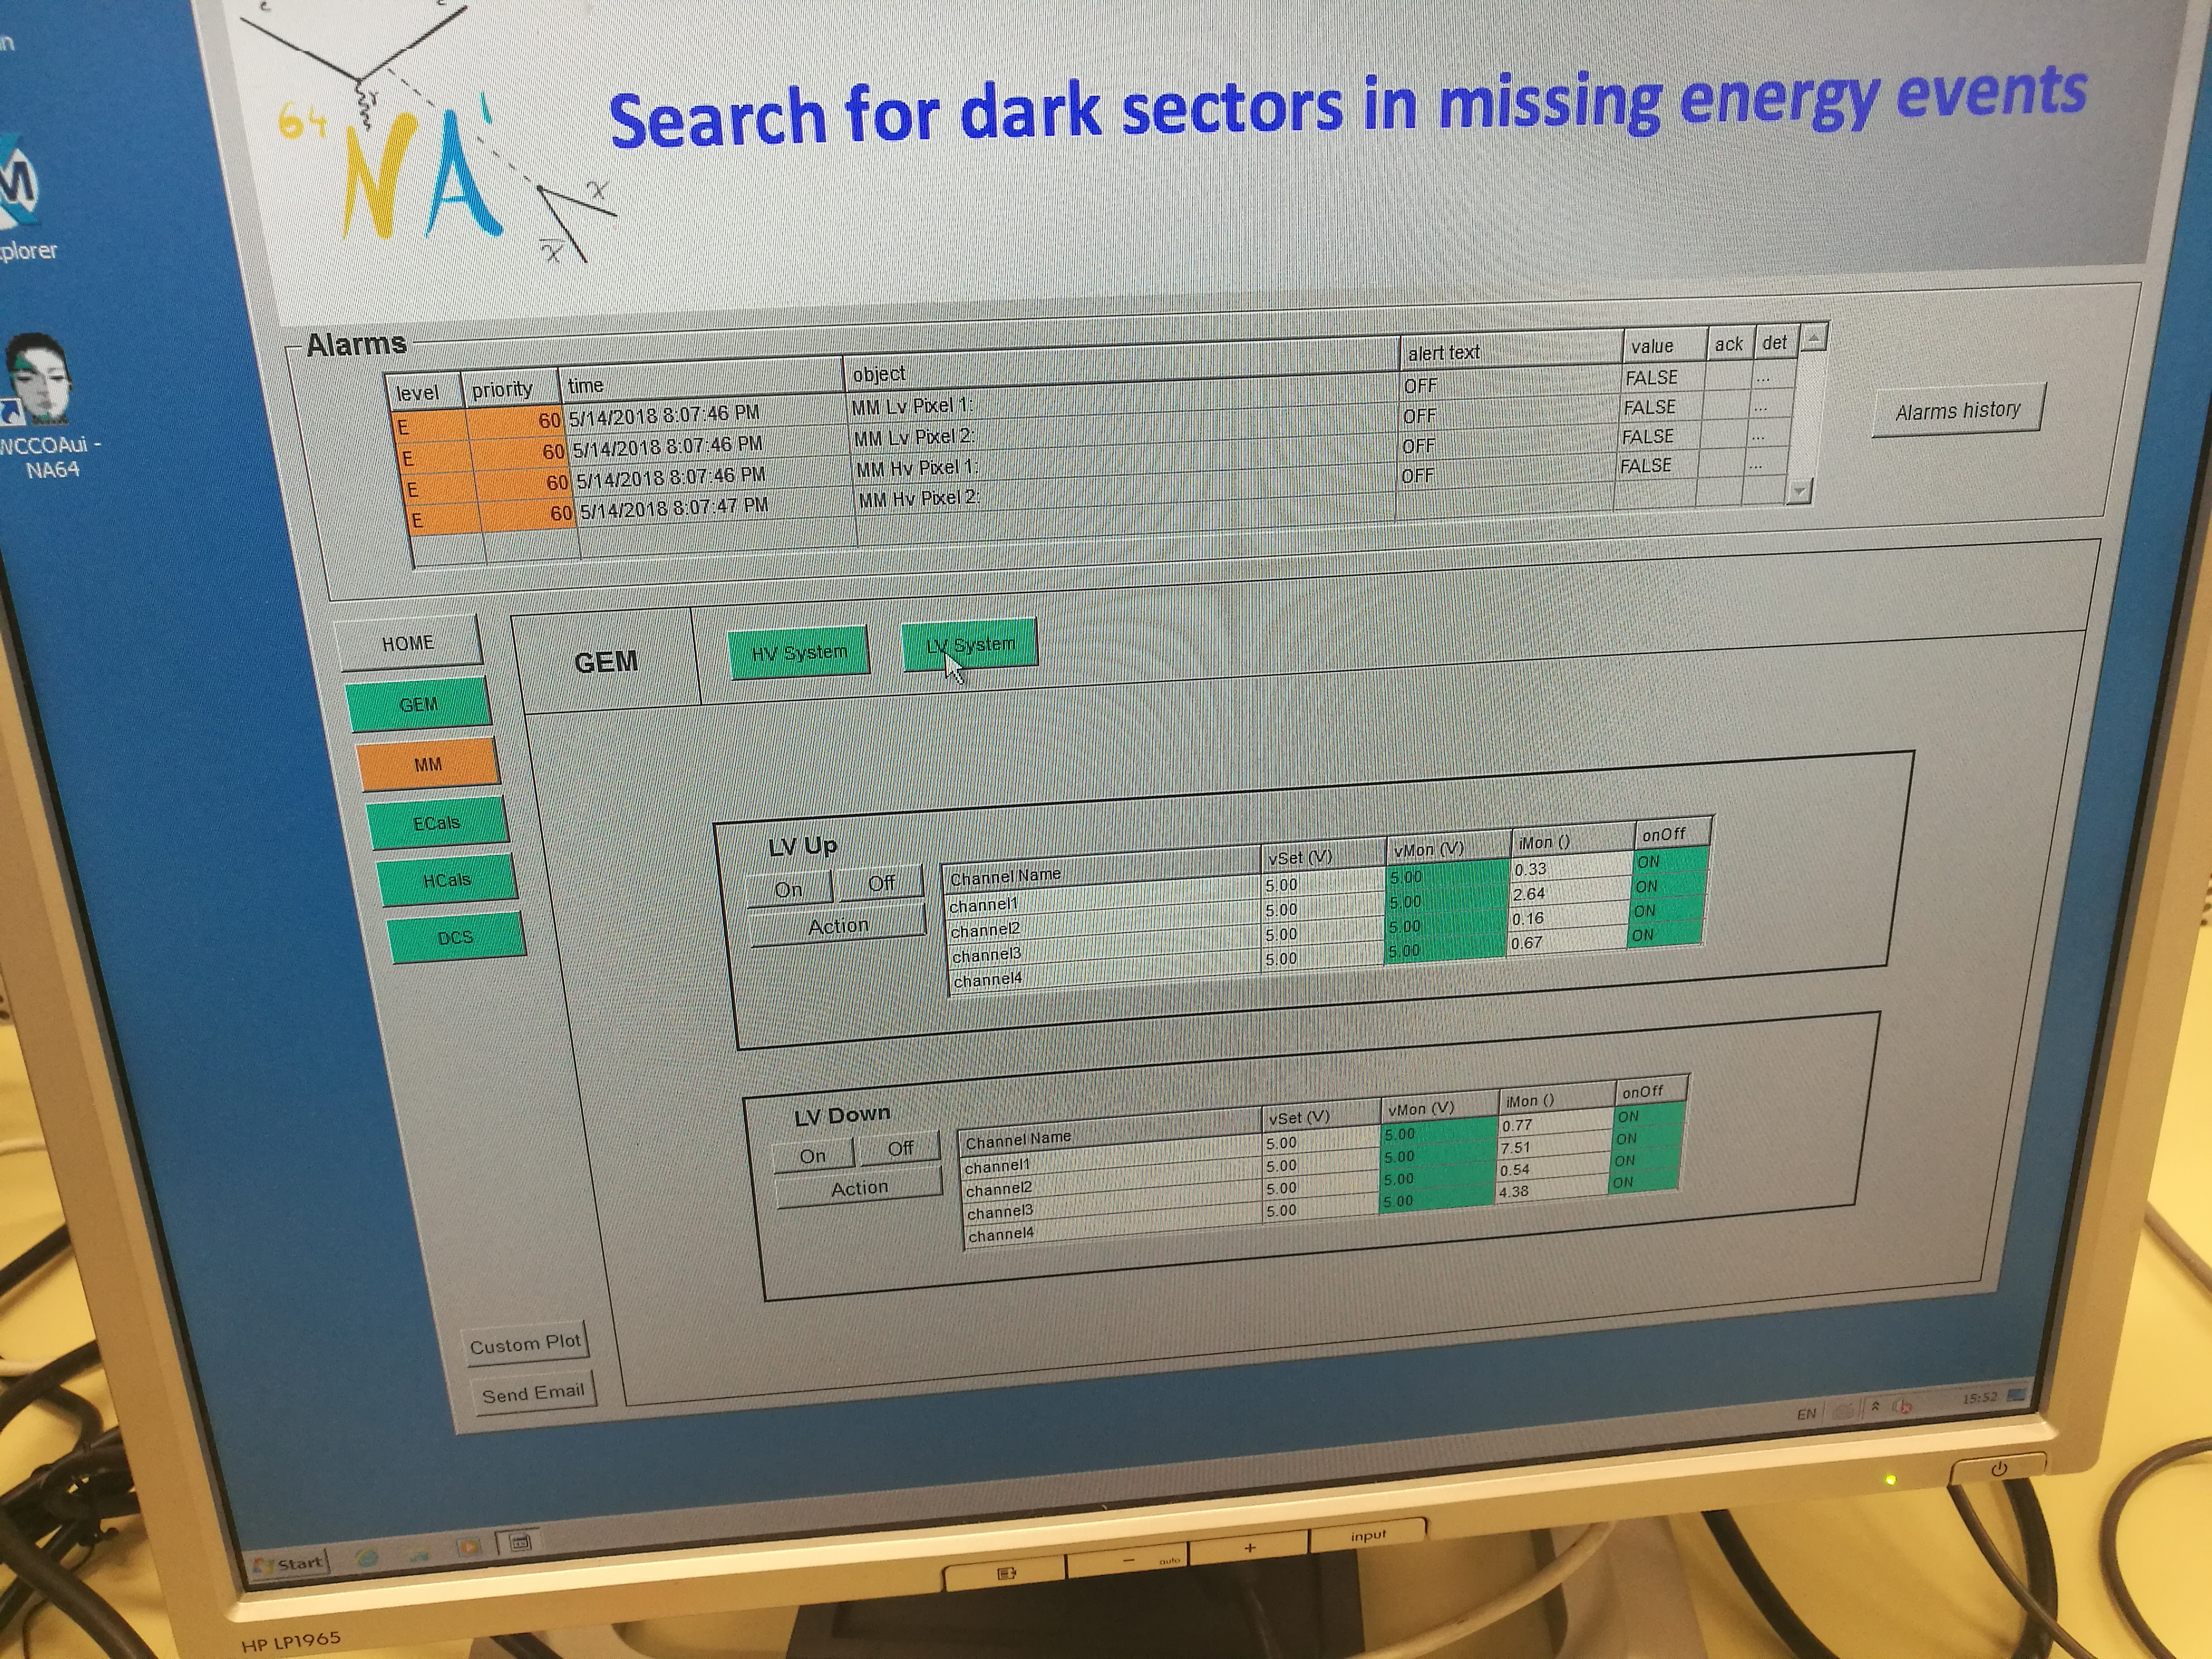
\includegraphics[width=.9\linewidth]{LV_SC.jpg}
\end{center}

\subsubsection{MM are loading but do not show up in COOOL}
\label{sec:org88f6e60}
the most probable cause is that those modules are not synchronized, typically happens to two of the Micromegas downstream either MM3,MM4 or MM5,MM6 will fail to show hits simultaneously.
The Module needs to be loaded again and then checked in COOOL. They might need a few try before they get all synchronized. Alternatively GemMonitor can be used to quickly test the response of the modules.
\subsubsection{MM are loading but show only noise or very low efficiency}
\label{sec:org944e3d4}
\begin{enumerate}
\item Check the voltages and current in HV strips in the slow control. 
Just click on the MM icon and HV strips on the window appeared. If one of the channel tripped an error message in red will be appeared in the message browser on the top window. One can try to
turn on the channel again, it is better to do it in two stages, first setting a voltage 20 Volt lower than the nominal one, turn on the Micromega, wait for the voltage to reach the selected value and then
set the nominal one. If unsure about this step contact one of Micromegas expert.

\textbf{Slow Control without problems:}

\begin{center}
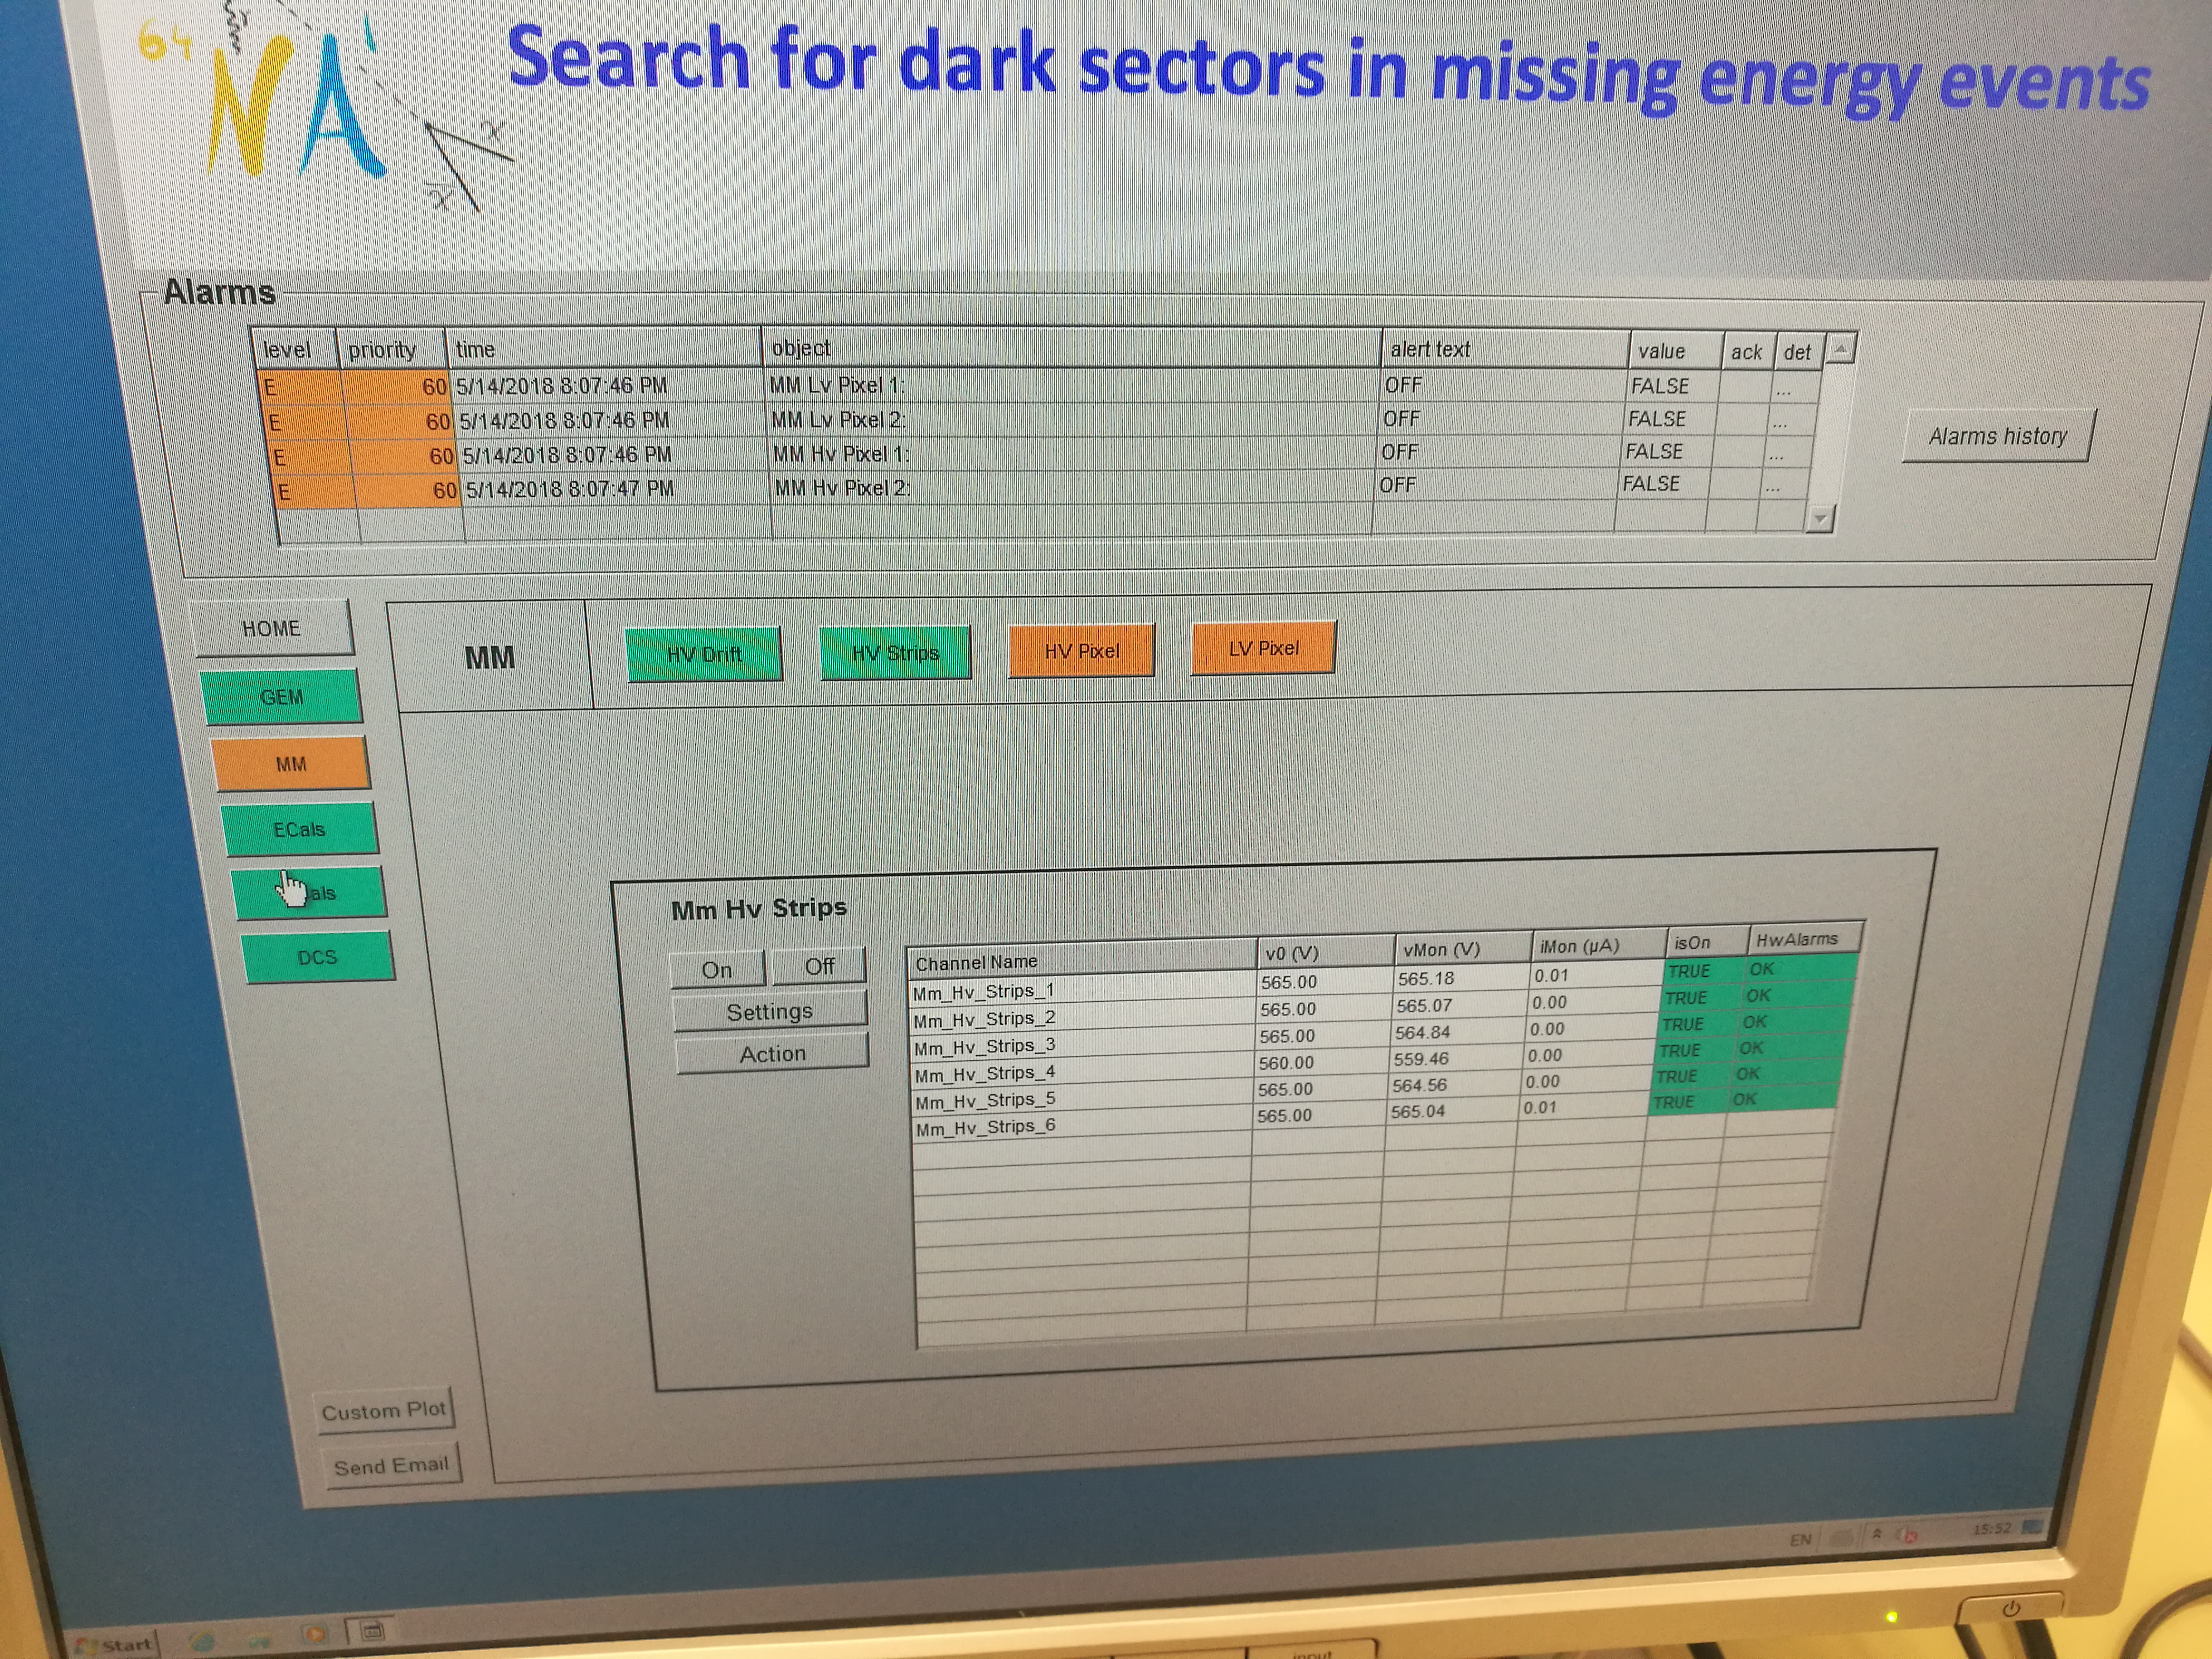
\includegraphics[width=.9\linewidth]{good_SC.jpg}
\end{center}

\textbf{Slow Control with tripped channel:}

\begin{center}
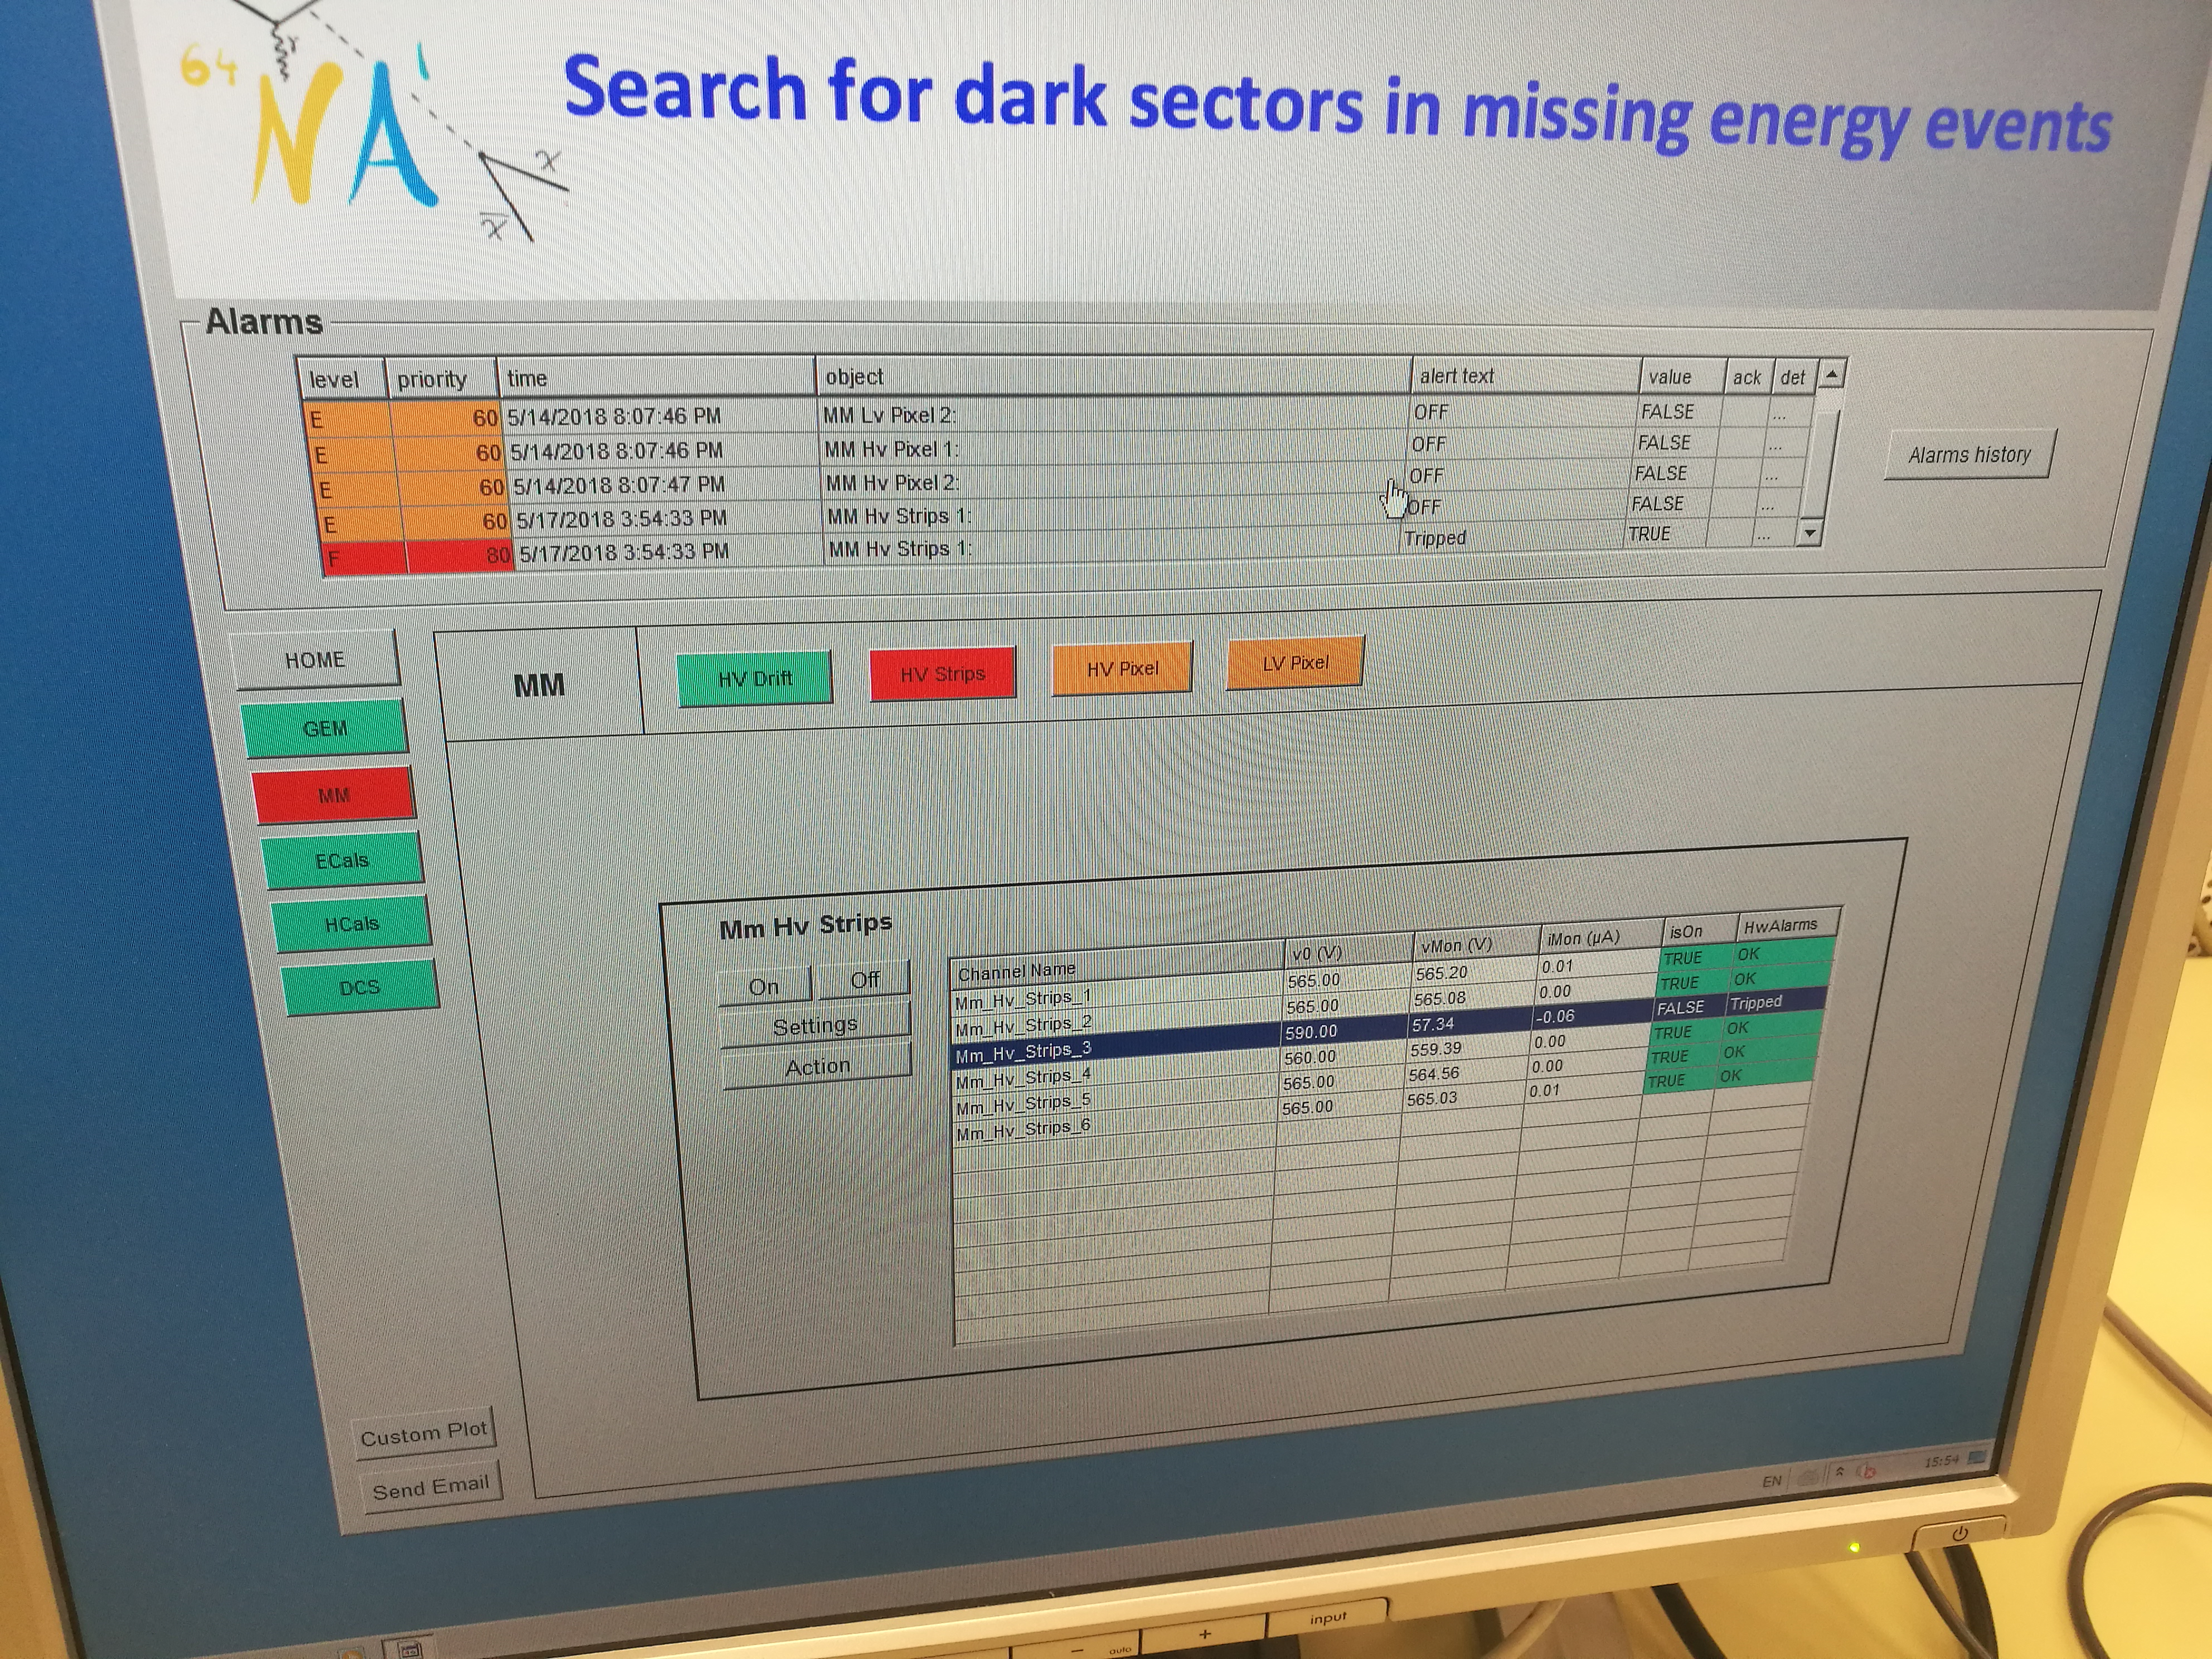
\includegraphics[width=.9\linewidth]{bad_SC.jpg}
\end{center}

\item If Voltages are okay but no current is shown during the spill check that the gas bottle has the correct pressure. If pressure on first regulator less than 0.5 bar contact one of Micromegas expert
immediately.

\textbf{Gas bottle with not enough pressure}

\begin{center}
\includegraphics[width=.9\linewidth]{inlet2.jpg}
\end{center}
\end{enumerate}

\subsection{Contacts}
\label{sec:orge84d9ea}
Emilio Depero
\begin{itemize}
\item \textbf{Mail}  : emilio.depero@cern.ch
\item \textbf{mobile} : +41 77 408 74 69
\item \textbf{mobile (only whatsapp or telegram)} :  +39 348 85 23 812
\end{itemize}

\textbf{ONLY IF NO ANSWER WITH THE FIRST NUMBER TRY:}
Dipanwita Banerjee
\begin{itemize}
\item \textbf{Mail}  : dipanwita.banerjee@cern.ch
\item \textbf{mobile} : +41 76 548 42 16
\end{itemize}
\end{document}